\chapter{Phase 1 --- Proof of Concept}
The goal of Phase 1, which spanned approximately the first month of my project, was to arrive at a proof of concept. This phase started at the beginning of the project with a discussion my supervisor, and the identification of my client. I proceeded by analysing the project requirements using autoethnographic methods, designing the system, and implementing the proof of concept. I then evaluated the merits, drawbacks, and next steps for the project by discussing the proof of concept system with my client. 

\section{Requirements Analysis}
\subsection{Autoethnography}
\label{sec:c1_autoethnography}
\begin{quote}
`Autoethnography is an ethnographic method in which the fieldworker's experience is investigated together with the experience of other observed social actors. \cite{autoethnography}'
\end{quote}

\noindent In this phase, I took an autoethnographic approach to requirements analysis and to design. As the `fieldworker', I drew on my own experience being involved in teaching Haskell as a teaching assistant for \hyperref[COMS10016]{COMS10016} for the last two academic years. This experience was very valuable to this project, and it allowed me take the initial brief from my supervisor and effectively design a solution, and then quickly implement a proof of concept of this solution. 

\subsection{The Brief}
This project was proposed by my supervisor, Jess Foster. In our initial meeting, we discussed how she wanted a tool that would help build intuition for how functional languages are evaluated, that she could use to supplement her explanation of otherwise difficult to intuit functional language concepts. We also discussed the benefits of the tool being accessible to students to use themselves during labs or at home. Jess helped me to identify an appropriate client: Samantha Frohlich. Jess and Samantha are both lecturers on \hyperref[COMS10016]{COMS10016}. It was necessary to identify a client other than Jess, as her existing role as my supervisor/primary marker could limit guidance she would be able to give me as my client. 

Following this meeting, I broke down this brief into smaller parts. Taking an autoethnographic approach, I used my own experience teaching functional languages to consider solutions, and what those solutions would entail, for each part of the breif. 

\subsubsection{Building Intuition}
\label{building_intuition}
This is the key to an effective solution. Most students of the first year \ac{FP} unit do not have any experience with functional programming before they take it. 
% \sam{I disagree with the rest, cos we strive for the lectures to be engaging (so maybe you can say that the teaching style is already to make learning not passive, so this will further that. Also your comment about not attending or engaging with labs is irrelevant cos if they dont engage with labs why would they use your tool? } 
% \todo{REWORK THIS PARA}
% and find it difficult to gain an intuition from passively watching lectures, and do not attend or engage with labs. 


% All participants who did not disagree that functional languages are hard to learn were presented with a free form text box, and asked to describe why. These responses were turned into a word cloud \ref{fig:fp_wordcloud}. Half of responses included the word `different'. 

In my experience teaching \ac{FP}, a very effective way to build intuition for functional programming languages is to demonstrate evaluation step by step. I frequently wrote out evaluations on paper for students during the \hyperref[COMS10016]{COMS10016} labs. I would also ask students to complete sections themselves. Others have also found that encouraging stepwise evaluation on paper is an effective way to get `a feeling for what a program does'~\cite{fp_first_year}.

Thus, a tool to perform these step by step evaluations in an interactive manner would be very valuable. The tool should have an interface that allows progress to be made step by step, showing the history of past steps as well as giving information about the step about to be taken. This would allow students to understand and interact with a stepwise evaluation, without anyone having to undertake the long process of writing it out, and without risk of incorrectness. Furthermore, the effects of changing the input program could be seen quickly, providing instant feedback. 

\subsubsection{Use as a Lecture Tool} The tool should be suitable for use in lectures. It should provide an interface that facilitates quality explanation of functional programming languages. The interface must be understandable, for both \ac{FP} `experts' (lecturers, advanced users) as well as people who have never seen a functional language before. 

\subsubsection{Use as a Self Teaching Tool} The tool should be `self-explanatory' enough for people to use it on their own without expert help. It should be fairly intuitive, and should have all the information required to use it presented to users. The tool must also be portable, and not require a complex installation process. The less complex this tool is to use, the more people will use it. 

\subsubsection{Demonstrating \ac{FP} languages} The tool must contain, at its core, a functional language in order to demonstrate how they work. Using a language that is similar to Haskell would make for easier evaluation of the project, as this would match the language taught in \hyperref[COMS10016]{COMS10016}, and therefore more people at the University of Bristol would be able to engage with the project. The most Haskell-like programming language that exists (as far as I am aware) is Haskell. 

Haskell could be included in the system/required to be installed on the host machine, however creating a demonstration tool around Haskell would be difficult due to the sheer size of the language, the number of features, and the complexity of the type system. It would be better to create Haskell-like language with a strictly limited size and include this in the system. The programming language should be designed with simplicity and clarity at its heart.

\subsection{SFL Explorer}
The requirements extracted from autoethnographic methods, as well as from my initial supervisor meeting, came together to form the idea for SFL Explorer. 

The system should be a website to maximize portability. The system should include a functional programming language, as well as some sort of UI that allows a functional program in the language to be entered, and evaluated step by step in a visual manner. 

% \begin{figure}[t]
%     \centering
%     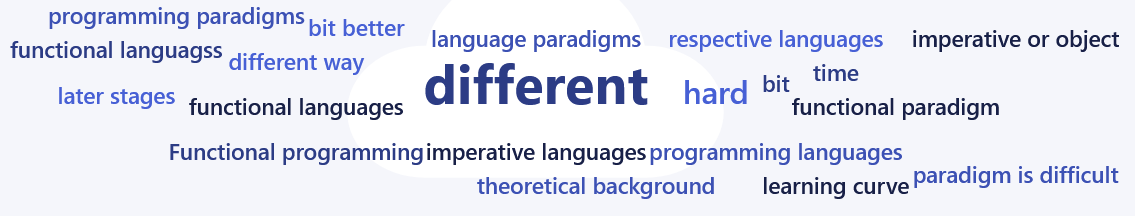
\includegraphics[width=1\linewidth]{images/fp_is_hard_wordcloud.png}
%     \caption{A word cloud of answers entered into the free form text box presented to the 10 respondents who reported that they did not disagree that functional languages were hard to learn}
%     \label{fig:fp_wordcloud}
% \end{figure}

\subsubsection{The Simple Functional Language}
\label{design:goals}
The language was given a name reflecting its core design principle: Simplicity. More precisely, the programming language should be designed with the following design principles in mind:
\begin{enumerate}
    \item \textbf{It should be simple and easy to understand}. This requires that the language should not have features that users might find difficult to understand why they work. This means that the language should have very few inbuilt functions, all of which should be easy to understand what they are for and what they do. 
    \item \textbf{It should be similar to existing functional languages}. This would allow users to be able to transfer their intuition to other languages and vise versa. It should be similar in syntax (it should have similar tokens and structures), as well as semantics (it should work similarly). 
    \item \textbf{It should be powerful enough to explain key concepts.}
\end{enumerate}
The features that should be selected for the language are the features that maximize these goals for the minimum implementation complexity. Out of our design goals, 2 and 3 have the potential to be in conflict, as more expressive power often requires more complex syntax. We must ensure a sensible compromise between all of our goals, while accounting for implementation complexity. When adding features for the language, we must prioritize the features that allow explanation of the `core' features of functional languages, and de-prioritise features that are not so `core' to the understanding of functional languages. 

\subsubsection{The Explorer}
The website (the explorer) should include a code editor for people to enter programs. Including the functionality for the language inside the website rather than requiring complex client/server communication would simplify the system, as well as improving responsiveness. 

\section{Language Design}
In this section, I will discuss the design of \ac{SFL} with respect to the requirements. This is iteration 1 of the design: the proof of concept.  

\subsection{Definitions}

% \sam{im so sorry but this looks ugly. I think it just needs more space, it is very crampt, this is a minor thing and can wait till the very end}

\subsection{Basic Syntax}
Lambda calculus is the basis of modern functional programming languages. As discussed in the background~\ref{bg:lcalc}, lambda calculus consists of 3 structures: identifiers, application, and abstraction. One common extra structure that functional languages implement is an assignment. This is where we label an identifier with a certain meaning, such that all references to the assignment henceforth are identical to a reference to the meaning assigned. For instance, the following two listings are semantically identical:
\begin{lstlisting}[language=SFL]
f = (\x.x)
main = f y
\end{lstlisting}
% \sam{dont do this, cos it gives latex the chance to mess up your formatting. Always give your listings a name and use the name in a full sentence e.g. "For instance, listing 1 and listing 2 are semantically equivalent"}
\begin{lstlisting}[language=SFL]
main = (\x.x) y
\end{lstlisting}
Note the use of \verb|"\"| instead of \(\lambda\) as it is the closest character available on most keyboards. A program is then defined as a set of assignments, and we pick one specific label name to mark the `entry-point' expression in the program. Haskell, as well as many other languages, uses `main' to represent a programs' entry point, so we may use main. 

Most programming languages, including functional ones, at least support integers. Booleans are also often supported to represent the results of integer comparison. Without literal values, programs would have to use complicated encodings (such as church numerals) to represent these values, making programs look more complicated.  We must also add a way to represent values, such as integers and booleans, to our language. 
These two features massively shorten and simplify programming in this language. Definition~\ref{sfl_basic_syntax} shows the basic syntax of \ac{SFL}. Expression syntax is the same as \lcalc, but with our literal values, and infix operators (such as +). A module is a set of assignments, and each assignments is a labelled expression.

% \sam{this is not referenced anywhere. Above you say we need x and then just dump x here. Instead motivate, introduce and explain. What additions have been made to execute x. Explain your definitions like you would explain your code}
\begin{syntax}[The basic syntax of \ac{SFL}]
(Lowercase Identifier): \(id ::= [a..z][a..zA..Z0..9\_]*\)\newline
(Operator): \(op ::= + \mid - \mid \times \mid / \mid > \mid \ge \mid < \mid \le \mid== \mid \mathrel{\mathtt{!=}} \)\newline
(Uppercase Identifier): \(Id ::= [A..Z][a..zA..Z0..9\_]*\)
\newline\newline\noindent
(Expression) \(E, F ::= [-][0, 1, ..]\mid E\; op\; F \mid true \mid false \mid id \mid \setminus id. E \mid E\:F\)\newline
(Assignment) \(A ::= id = E\)\newline
(Module) \(M ::= A\: M \mid End\)
\label{sfl_basic_syntax}
\end{syntax}

% \subsection{Design: Reduction and Progress} ???


\section{Implementation}
\subsection{The Abstract Syntax Tree}
% The tree structure of \ac{SFL} requires the following different types of tree nodes:
% \begin{itemize}
%     \item Identifier
%     \item Literal
%     \item Application
%     \item Abstraction
%     \item Assignment
%     \item Module
% \end{itemize}
% \sam{bullets look silly, if you have spare time draw a pictures, otherwise just say that it is a tree structure, listing the nodes adds nothing}

Programming language syntax can be expressed in a tree structure, known as an \ac{AST}. The process of turning a program from a string to a tree is known as parsing. In order to effectively explain the structure of a parsed program going forwards, the following structure will be used to give a written representation of an \ac{AST}:
\begin{itemize}
    \item Nodes are represented as one line each, where, with the name of the node type, followed by its value for \verb|Literal|s and \verb|Identifier|s.
    \item The children of a node are all of the nodes with an indentation level one deeper than the node in question listed directly below it, until a shallower or equal depth node is listed. 
\end{itemize}

\noindent
For instance, 
\begin{lstlisting}
main = (\x.1) 2
\end{lstlisting}
would be represented as:
\begin{lstlisting}
Module:
  Assignment:
    Identifier: main
    Application:
      Abstraction:
        Identifier: x
        Literal: 1
      Literal: 2
\end{lstlisting}
Initially, the approach taken when implementing this tree structure was to have each node `owning' its child nodes (see \ref{bg:rust}). However, it will be frequently necessary to be able to find nodes based on certain conditions (for example, the condition that this node is a valid redex) and then provide a value that represents the location of this node within the tree. Even if each of the tree nodes had a unique ID, locating a node from this value representing its location will require some sort of tree search.

Rather than this solution, which would have a non-constant node lookup time, a secondary structure can be used to store the tree nodes with constant time lookup, and then each node can store a value enabling constant time lookup of its children within this structure. In the implementation, these types were labelled as \ac{AST} and ASTNode, where \ac{AST} was an array of ASTNodes, and each ASTNode stored their children's indices in this array. The position in the array of an ASTNode will be referred to as its index.

See \ref{fig:ast_lst} for the code listing for the \ac{AST} definition. In this implementation, \verb|Vec| was used for the array, as it is growable, resizeable, and facilitates constant-time lookup of its elements. The \ac{AST} stores and owns all of the nodes, as well as storing the index of the root node rather than requiring it to be at a specific index. 

The node indices in the \verb|children| vector represent different things depending on what kind of node it is. 
\begin{itemize}
    \item If it is an abstraction, the first node represents the variable (or pair of variables) abstracted over, and the second node represents the expression.
    \item If it is an application, the first node is the function, and the second is the argument.
    \item If it is a module, then each of the children is an assignment.
    \item If it is an assignment, then the first child is the variable being assigned to, and the second is the expression.
\end{itemize}

\verb|Literal| and \verb|Identifier| nodes store the tokens that defined them, so the strings can be accessed. \verb|Identifier| nodes used as abstraction arguments. These types can either be specified in the source program, or inferred later. Nodes also store their positions (line and column) in the source program, which can be used for error messages. 

\begin{figure}[t]
    \centering
    \begin{tabular}{c}
    \hline
    \begin{lstlisting}[language=Rust]
struct AST {
    vec: Vec<ASTNode>,
    root: usize,
}

enum ASTNodeType {
    Identifier,
    Literal,
    Application,
    Assignment,
    Abstraction,
    Module,
} 

struct ASTNodeSyntaxInfo {...}

struct ASTNode {
    t: ASTNodeType,
    token: Option<Token>,
    children: Vec<usize>,
    line: usize,
    col: usize,
    type_assignment: Option<Type>,
    additional_syntax_information: ASTNodeSyntaxInfo
}
    \end{lstlisting}
    \\\hline
    \end{tabular}
    \caption{The Rust code listing for the definition of the AST, with lifetime specifiers, accessibility modifiers, and the syntax information (see \ref{paragraph:to_string}) removed for conciseness.}
    \label{fig:ast_lst}
\end{figure}


\subsubsection{With the Benefit of Hindsight} % for jess's benefit as she did not like my AST definition so i want to aknowledge what she said about it
% \sam{very nice evaluation, love this section}
This project was my first major project using Rust. Below is a discussion of some Rust features which were not fully taken advantage of in this definition of syntax trees, followed by a discussion of a combination of these features that would have been more optimal. 

\paragraph{Tagged Unions}
An alternative implementation could have involved \verb|ASTNodeType| being a tagged union, with different node types being associated with different children and data items. For instance, application could be represented by \verb|Application(f: usize, x: usize)|, and identifiers could be \verb|Identifier(String)|. This would be more space efficient, as each node requires different data, and we would no longer need to store empty fields for data items we do not need. It would also more elegantly represent the fact that each type of node is a different `thing', and de-obfuscate the meaning of each of the different fields of a node. 

\paragraph{References}
This definition of the \ac{AST} has a parent object (the \verb|AST|) owning all of the nodes (the \verb|ASTNodes|). As previously discussed, this was done to enable constant-time lookup of nodes from their indices. However, all things in a program already have such a reference enabling constant time lookup: a pointer, represented in rust by a reference. This was not used, as there were concerns about ensuring validity of each reference, and avoiding use-after-free bugs. These concerns were unfounded, as one of Rust's major features is that it provides safety guarantees ensuring that these problems are never encountered \cite{rust_book}. An object can only store a reference to another object if it can be guaranteed that it exists, and it will continue to exist for at least as long as the object storing the reference will. This is achieved via lifetime checking, using either inferred or explicitly stated specifiers of how long the two objects will exist relative to each other. 

\paragraph{A Better Implementation}
Figure \ref{fig:ast_lst_2} shows an implementation that uses tagged unions to store information that is different for different node types, and pointers to the nodes directly rather than list indices. This avoids the possibility of referencing nodes that don't exist. It is also easier to understand what is common between nodes (syntax info) and what is uncommon. It is also more space efficient as it only stores the information that each type requires. The size of the improved implementation is 88 bytes, and the size of the original implementation is 128 bytes. The improved implementation is subjectively more elegant and readable. Objectively, it also takes up less space. It also forces memory safety, without the need for carefully implemented getter and setter functions. 

Despite this, the decision was made not to update the implementation for several reasons. The \ac{AST} is so central to the implementation, that it would take a long time to switch properly. Memory and speed are not major constraints for this project, but implementation time is. Furthermore, as long as all indices used are either produced by a helper function, or the \ac{AST} root, there should not be a problem with memory safety. 

\begin{figure}[t]
    \centering
    \begin{tabular}{c}
        \hline
    \begin{lstlisting}[language=Rust]
struct AST<'a> {
    vec: Vec<ASTNode<'a>>,
    root: &'a ASTNode<'a>,
}

enum ASTNodeType<'a> {
    Identifier{name: String},
    Literal{value: String, _type: PrimitiveType},
    Assignment{to: String, expr: &'a ASTNode<'a>, type_assign: Type},
    Abstraction{var: String, expr: &'a ASTNode<'a>, type_assign: Type},
    Module{assigns: Vec<&'a ASTNode<'a>>},
} 

struct ASTNodeSyntaxInfo { ... }

struct ASTNode<'a> {
    t: ASTNodeType<'a>,
    info: ASTNodeSyntaxInfo
}
    \end{lstlisting}
    \\\hline
    \end{tabular}
    \caption{An alternative implementation with a few advantages over the actual implementation. }
    \label{fig:ast_lst_2}
\end{figure}

\subsection{Methods on the AST}
Below are a selection of the more important or interesting methods implemented on the \ac{AST} and its nodes. \sam{i think I want to see the code as well}

\paragraph{Adding new nodes} We will frequently want to add new nodes to the tree. Where they are inserted is not important, so the tree will add them to the end, and return their index. These methods are needed extensively for the parser.

\paragraph{Getting children of nodes} As the interpretation of the \verb|children| array for each node changes depending on what type of node it is, a series of getters are implemented, such as `\verb|get_func|' to get the function of an application. These methods are needed extensively for the type checker, and the redex finding system. 

\paragraph{Substitute variable} Substitutes all instances of a variable in an expression with a given expression. This is needed for applying abstractions. For instance, the process of reducing \verb|(\x.x) 1|, is:
\begin{itemize}
    \item Get the name of the variable abstracted over: \verb|x|.
    \item Replace all instances of x in the abstraction expression with the right hand side of the application: \verb|1|.
    \item Replace all references to the abstraction with references to the abstractions expression. 
\end{itemize}

Note that this orphans the node for the abstraction, and the node for the abstraction variable \verb|x|. This is hard to rectify as deleting any nodes will shift the whole list, which would invalidate indies of nodes, which will break many of the references. This is rectified by cloning the AST, as described below.

\paragraph{Clone} The AST, or just a subsection of the \ac{AST} from a given node, can be cloned by starting from the desired new root, and cloning each nodes children recursively. The new indices of each node may not be the same, as they may be moved in the list, but they will all be in the same place relative to each other. This also removes orphaned nodes, as they will never be cloned as they have no parents. 

\paragraph{To String} \label{paragraph:to_string} Programs can also be effectively transformed back into strings. This requires a few other pieces of information to be associated with some tree nodes, to make the output program as similar to the input program as possible. The more similar the output is to the input, the easier it is to understand. Some examples include:
\begin{itemize}
    \item Whether the application was generated by using the right associative \verb|$| operator in order to avoid parenthesis, for instance \verb|id $ 1 + 1|. 
    \item Whether the assignment, where the expression is an abstraction, was generated using the syntax \verb|x = \a.e| or the syntax \verb|x a = e|. 
\end{itemize}
We must also take into account whether a binary infix operator was used to generate a function call, and if so we must place it in the middle of its arguments. 

% There is also other syntax sugar, such as turning a List from `Cons' syntax into more familiar braced syntax, with comma separation.   For instance: \verb|Cons 1 (Cons 2 (Cons 3 Nil))| should be displayed as \verb|[1,2,3]|. [TODO: Consider whether to have only literals in this syntax or everything. Maybe toggleable syntax sugar?]


\subsection{The Parser}
The parser needs to consume a program, and return the AST. It can also disqualify some invalid programs while generating the tree, rather than having to traverse it after generation to catch these issues. For instance, we must the following assignments:
\begin{itemize}
    \item \verb|x = (\x. e)| where e is a valid expression, as x is ambiguous during the expression e. This would be disqualified when attempting to parse the abstraction as x is already bound.  
    \item \verb|x = y| where y is undefined.
\end{itemize}

% \sam{some advice i got when i started technical writing, as i think you are writing very similarly to  how I used to: when writing a report it is tempting to well report "this was done" "that was done" "this means" "noun will need to" but this results in quite dry and overly verbose writing. Instead it is more exciting to make the research / the noun the subject of the sentence. e.g. "noun needs to bla because of bla"}

\subsubsection{Lexical Analysis}
Lexical analysis is the process splitting a program into its constituent tokens (Lexemes). For instance, the program \verb|main = (\x.x) 1| is the following stream of tokens: \[[Id: main, Assignment, LeftParen, Backslash, Id: x, Dot, Id: x, RightParen, Literal: 1]\]
See \ref{appx:tokens} for the full code listing of the definition of the tokens output by the lexical analysis, including syntax that was added in phase 2 that we have not discussed yet.

The lexer loads the entire string into memory at once. This is not typically best practice, as this can lead to problems with lexing large files. The approach discussed in \cite{dragon_book} which I normally take when writing lexers relies on a system of two buffers only holding individual pages of the file from disk. However, this system will not be loading files from disk; the program string is already in memory as it comes from the UI. 

The lexer provides a \verb|next_token| function that returns the next token, and advances the pointer to the start of the string. The lexer keeps track of line and column information, which is stored in the token to then be stored in the AST. 

\subsubsection{Expression Parsing}
Expressions are parsed using recursive descent parsing. Some of the techniques used for this part of the parser were inspired by the discussion of top down parsing in \cite{dragon_book}. 

At the top level, the expression parsing method is \verb|parse_expression|. A variable \verb|left| stores what is currently the index of the expression parsed so far. It is called \verb|left| as if we encounter a token that denotes that \verb|left| is applied to whatever comes next, it becomes the left hand side of the application. \verb|left| is originally set to be the output of parsing a primary (see \ref{impl:parsing_primary}). Following this, parsing progresses differently based on the next token. Below are some of the ways that \verb|parse_expression| could proceed.
\begin{itemize}
    \item If the next token is an open bracket, we consume the token and then parse an expression. We then expect a closing bracket. We set \verb|left| to the application of the current value of \verb|left| to the expression.
    \item If the next token is a dollar sign, we consume the token and then parse an expression. We do not expect a closing bracket, and we error if we receive one.  We set \verb|left| to the application of the current value of \verb|left| to the expression, marked with a flag saying that the application was generated by a dollar sign (see \ref{paragraph:to_string} for how this is used).
    \item If the next token is a token denoting the start of a primary expression, such as:
    \begin{itemize}
        \item A backslash, indicating the start of an abstraction.
        \item An identifier, indicating a variable.
        \item A literal.
    \end{itemize}
    We parse a primary, and set \verb|left| to the application of the current value of \verb|left| to our primary.
    \item If the next token is a token indicating the end of an expression, such as:
    \begin{itemize}
        \item A closing bracket
        \item EOF
        \item A newline
        \item A double colon, indicating a type assignment follows
    \end{itemize}
    We return \verb|left|. 
\end{itemize}

\paragraph{Primary Parsing}
\label{impl:parsing_primary}
A primary is a less complex structure than an expression. In this system, a primary is any expression structure other than applications. The primaries are:
\begin{itemize}
    \item Literals
    \item Identifiers
    \item Abstractions
    \item Expressions in brackets
\end{itemize}
Each of these have their own specific parsing algorithms, which may include calling \verb|parse_expression|. 

\paragraph{Literal and Identifier Parsing}
Literals and identifiers are turned trivially into their respective AST Nodes. For instance, the token:
\begin{lstlisting}[language=Rust_boxed]
Token {
    line: 0,
    col: 0,
    tt: TokenType::IntLiteral
    value: "2"
}
\end{lstlisting}
Is turned into this ASTNode:
\begin{lstlisting}[language=Rust_boxed]
ASTNode {
    t: ASTNodeType::Literal,
    token: Some({the token}),
    children: [],
    line: 0,
    col: 0,
    type_assignment: Option<Primitve::Int>,
    additional_syntax_information: ...
}
\end{lstlisting}

\noindent To parse an identifier, we must also check that the identifier is bound at this location.

\paragraph{Parsing Abstractions}
Abstractions (in the simple case) are parsed by:
\begin{itemize}
    \item Consuming a lambda (represented by `\verb|\|' for ease of typing on standard keyboards).
    \item Parse a variable. This variable must be added to our set of `bound' variables.
    \item Consuming the dot separator`\verb|.|'.
    \item Parsing an expression.
    \item Constructing an abstraction node from the variable and the expression.
\end{itemize}

\noindent Abstractions have a few complicating elements of syntax sugar.

\subparagraph{Abstractions May be Assignments}
The assignment \verb|f x = x| is implicitly \verb|f = \x. x|. This is solved by parsing an argument to \verb|parse_abstraction| representing whether this is an assignment. If it is an assignment, we expect the assignment operator `\verb|=|' as our separator between arguments and term rather than the dot. As previously mentioned in~\ref{paragraph:to_string}, in order to output the string in a format that is as close as possible to the input, we set a flag in the \verb|ASTSyntaxInfo|: \verb|assign_abst_syntax| to all abstraction nodes defined like this. 

\subparagraph{Abstractions May Have Multiple Variables}
The abstraction \verb|\x y. x| is syntax sugar for \newline\noindent\verb|\x. (\y. x)|. Additionally, with the abstraction-assignment syntax, \verb|f x y = x| is syntax sugar for \newline\noindent\verb|f = \x. (\y. x)|. This can be accounted for by continually parsing variables until we encounter `\verb|.|' or the assignment operator `\verb|=|', and then producing a series of nested abstractions over these variables in order. 

\subsection{Making Progress}
\label{c1_design_reduction_progress}
Functional programs progress via reduction. \lcalc\ expressions can reduce when we have an abstraction applied to a term. This is much the same in \ac{SFL}, the difference being we can also apply labels representing abstractions to terms. In the following listing, expressions labelled as `\sflinline{main1}' and `\sflinline{main2}' both reduce to \sflinline{5}. 
\begin{lstlisting}[language=SFL]
f x = 5

main1 = f 10 
main2 = (\x. 5) 10
\end{lstlisting}
\noindent Rather than simply reducing `\sflinline{f 10}' to 5 in one step, it would be useful to show the substitution to help users to understand why `\sflinline{f 10}' becomes `\sflinline{5}' here. This would involve substituting the variable \sflinline{f} for the function \verb|(\x. 5)|. We have two types of progress: reduction and substitution. In this section, we shall broaden the term `redex' to include both. 

\paragraph{Representing and Applying Redex-Contraction Pairs}
We can define a structure representing progress for our \ac{AST}: a pair where the first element is the node in the tree to be replaced, and the second element is an entirely new tree to replace it with. Below is how this type is represented in Rust. 
\begin{lstlisting}[language=Rust_boxed]
type RCPair = (usize, AST)
\end{lstlisting}
\noindent To do the substitution, we combine the two \ac{AST}s by concatenating their two lists of nodes, and replace all references to the original node to the root of the replacement \ac{AST}. This orphans the original node, as there is no references to it. Rather than simply deleting it, which would cause the list to shift and therefore invalidating the indices, we can clone the tree (see~\ref{}). 

\subsubsection{Finding Redex-Contraction Pairs in a Term}
\paragraph{Is the Term $T$ a Redex?}
The core of the redex finding algorithm is being able to identify whether a term $T$ with \ac{AST} index $P$ is a redex, and get its contraction. This is achieved by proceeding case wise on the shape of $T$.
\begin{itemize}
    \item $T = (\backslash x. M)\, N$: We construct an \verb|RCPair| where the left size is $P$, and the right side is the body of the abstraction $M$ with all instances of $x$ replaced with $N$. 
    \item $T = f$: We construct an \verb|RCPair| where the left size is $P$ and the right-hand side is the value associated with the identifier \verb|f| cloned into a new \ac{AST}. 
    \item Any other shape, $T$ is not a redex. 
\end{itemize}

\paragraph{Getting a List of Redexes in the Term $T$}
We first check if $T$ is a valid redex, and if so add it to our list. If $T$ is an application we extend this list with the lists of \verb|RCPair|s in the function and argument of the application. 

\subsection{Web UI \ac{MVP}}
As part of this section, I also developed the MVP for the Web UI. \ref{fig:screenshot_phase_1_end} shows the web UI after this stage of the project. 

\begin{figure}[h]
    \centering
    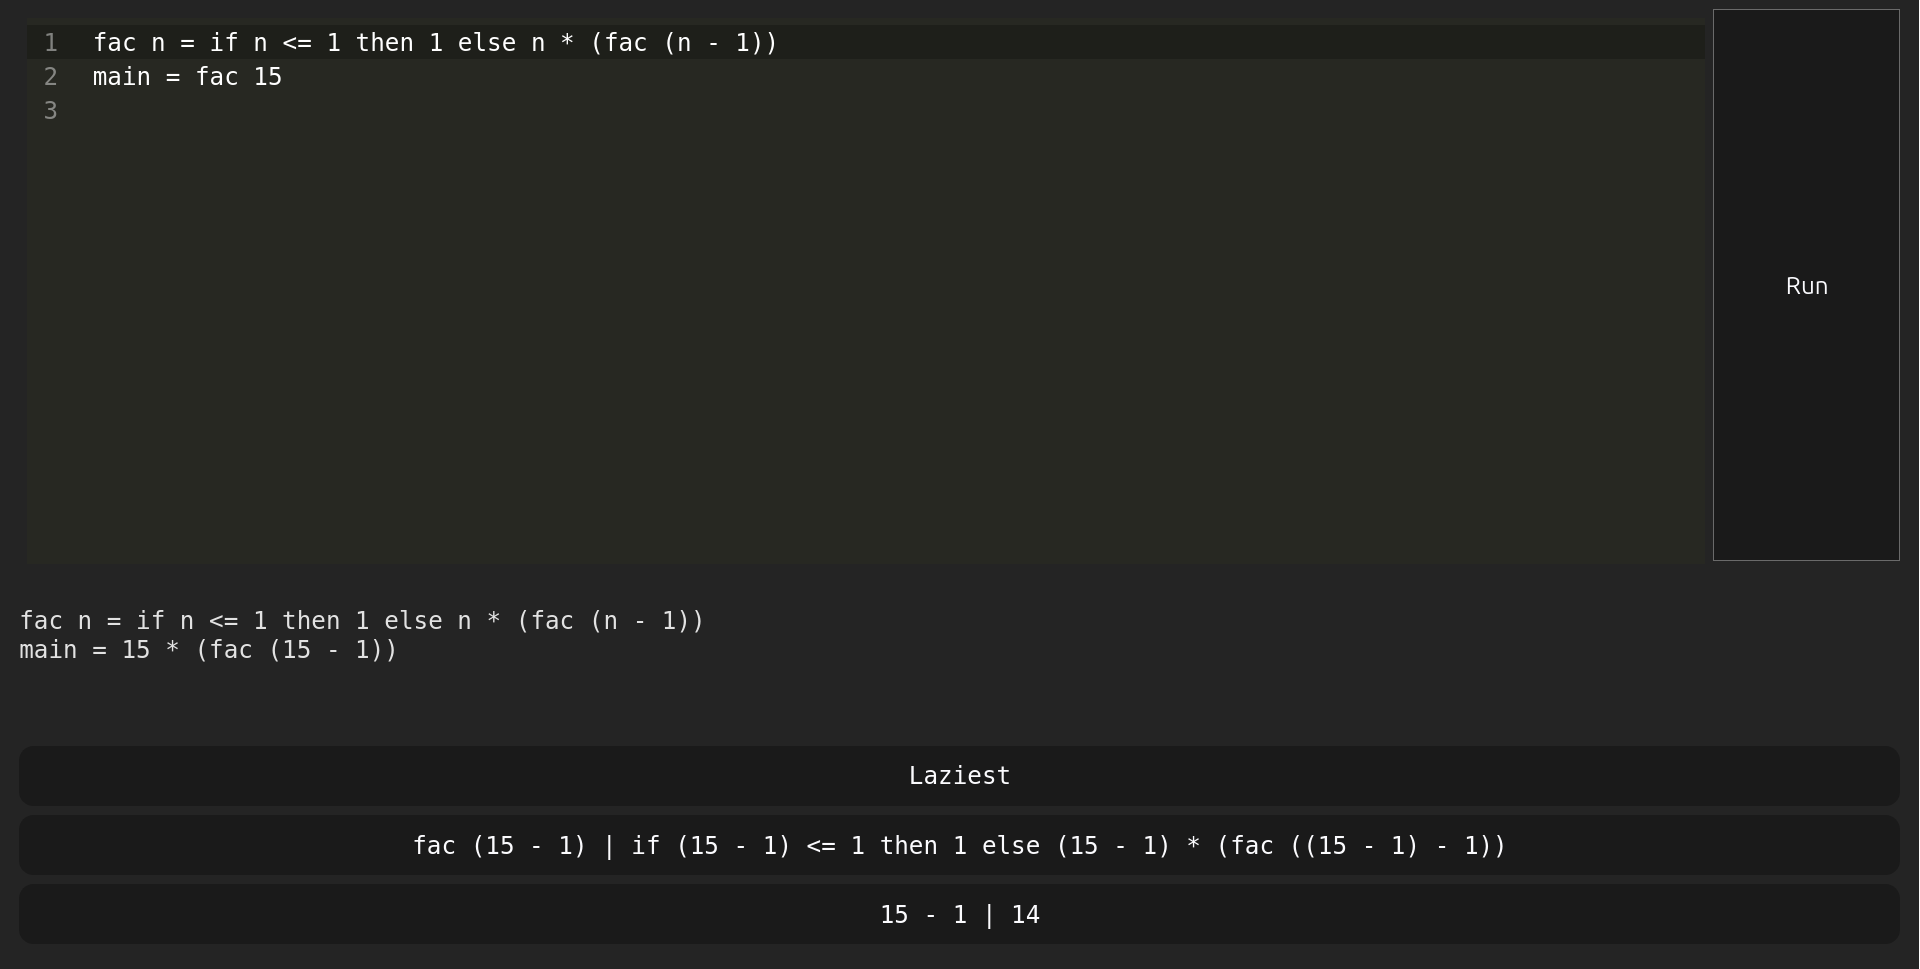
\includegraphics[width=1\linewidth]{images/phase-1-end.png} 
    \captionsetup{justification=centering}
    \caption{The Web UI \ac{MVP}, as presented to my client at the end of phase 1.}
    \label{fig:screenshot_phase_1_end}
\end{figure}

Until this point, development was done in one rust package. This package would be compiled to a binary and run natively, with a basic \ac{CLI}. This needed to be changed so that it can compile to \ac{WASM} and run in the web browser. As I wanted to keep the \ac{CLI} for debugging, I did not want to change the whole project to a project with a \ac{WASM} interface. A solution to keeping both interfaces was to separate the functionality that would be common to the \ac{CLI} as well as the \ac{WASM} library into a separate library, and then have the two interfaces as separate packages that depended on this one. The structure of the project became the following 4 packages. 

\begin{itemize}
    \item \textbf{libsfl}: All of the language functionality, as this is common to both interfaces
    \item \textbf{sflcli}: All of the original CLI functionality without the language functionality.  
    \item \textbf{libsfl\_wasm}: a package set up for use with wasm-pack (\ref{bg:wasm-pack}). It provides a wrapper around \textbf{libsfl}, with wrapper functions returning data structures supported by wasm-bindgen\ref{bg:wasm-bindgen}. wasm-pack would compile this to an \ac{NPM} package containing:
    \begin{itemize}
        \item The WASM binary blob of the compiled rust code.
        \item A JavaScript file that would load the blob into the browsers' memory, and that provides methods that can call the appropriate the methods in the blob.
        \item A TypeScript file providing the types of all of the packages exported functions. 
    \end{itemize}
    \item The Vite+React frontend (see \ref{bg:frontend}) that requires the package that results from compiling \textbf{libsfl\_wasm}.
\end{itemize}

The \ac{WASM} library provided functions that could be called from the JavaScript module. Rather than passing the \ac{AST} between the \ac{WASM} library and the JavaScript module, the \ac{AST} was stored at a known memory address, and retrieved during subsequent calls to \textbf{libsfl\_wasm} functions. 

\section{Proof of Concept Client Meeting: Evaluation and \newline Next Steps}
\label{eval:c1_client}
At the end of the phase, I presented the proof of concept project to my client, who was very positive about the project and its potential. The discussion was informal, a friendly conversation rather than a structured interview, to allow the direction of questioning to change depending on the client's answers. The meeting started with me giving my client a demo of the proof of concept, using the system to evaluate the following program:
\begin{lstlisting}[language=SFL]
fac n = if n <= 1 then 1 else n * (fac (n - 1))
main = fac 5
\end{lstlisting}

\noindent Below is a summary of my client's thoughts about various aspects of the proof of concept system and areas that could be iterated on.

\subsection{Usefulness as a Teaching Tool}
Below are some notes on what the client thought about the effectiveness of the project as a teaching tool, and how it could be improved in future iterations.
The project is already very useful as a teaching tool to demonstrate:
\begin{itemize}
    \item Evaluation order, and the importance of laziness.
    \item Currying.
    \item Recursion.
    \item The \lcalc.
\end{itemize}

\noindent On top of this my client wanted to be able to use the system to demonstrate $List$s and common $List$ functions such as `map' and `fold'. These do not have to by polymorphic, they could be just defined over $Int$s or some other type. These also do not need to be user-definable, they can be built in. However, supporting polymorphic user defineable data types would be very useful and much clearer. 

\subsection{The Existing Language}
\paragraph{Positives:}
\begin{itemize}
    \item The language looked similar to Haskell. Particularly, the \verb|if _ then _ else| syntax, and the function assignment shorthand syntax (\verb|fac n = ...| rather than \verb|fac = \n. ...|, even though these are identical)
    \item The language is minimal and clear
    \item The factorial function was quite elegant, and it would be understandable to people who did not know Haskell.  
\end{itemize}

\paragraph{Negatives:}
My client had no specific complaints about the language as it currently stands, however we agreed was lacking many important features. The most difficult things to teach are concepts involving more complex data types. 

\paragraph{Requested Features:}
Below are the specific features my client asked for in order for the system to be able to demonstrate the things she wants to use the system to demonstrate:
\begin{itemize}
    \item Recursive Types
    \item Polymorphism
    \item Type Aliases
    \item Typechecking
    \item User Definable Data Types
\end{itemize}

\subsection{The Existing UI/UX}
\paragraph{Positives:}
\begin{itemize}
    \item The editor, as it feels like a very popular editor: VSCode
\end{itemize}

\paragraph{Negatives}
\begin{itemize}
    \item It is unstable. This is bad in a teaching tool, as it would waste a lot of time if it constantly broke in the lecture. 
    \item `laziest' as an option is confusing, as it was unclear if it was referring to one of the other on screen options, or if it was referencing a `hidden' option
    \item The vertical bar separating redex from contraction on the progress buttons was not obvious enough. On top of this, the bar was not centred, so it was hard to look through all the redexes at once as they were not aligned with each other. 
\end{itemize}

\paragraph{Requested Features}
\begin{itemize}
    \item Syntax highlighting, to make the language easier to read   
    \item A history of what the expression has been is vital to demonstrate step by step evaluation. I identified this as an important feature at the beginning of the phase (see \ref{building_intuition}), but I had not finished it by the client meeting. It was implemented in the next phase (see \ref{c2_poc_ui_impl}). 
    \item Sample Programs
\end{itemize}

\subsection{Conclusion}
At the end of this phase, and going into phase 2, I had a strong proof of concept system and an idea for how the system will look. The meeting with my client yielded many ideas, all of which I sucessfully implemented throughout this project. 